% !TeX program = lualatex
% !TeX root = luaking.tex
% !TeX encoding = UTF-8
% !TeX spellcheck = cs_CZ
%---------------------------------------------------------------------------------------------------
% file fey1ch36.tex
%---------------------------------------------------------------------------------------------------
%=========================== Kapitola: Mechanizmus vidění ==========================================
\setchaptertoc
\chapter{Mechanizmus vidění}\label{fyz:IchapXXXVI}
  \section{Barevný vjem}\label{fyz:IchapXXXVIsecI}
    Při studiu pocitu vidění si musíme uvědomit, že nevidíme náhodné barevné nebo světelné skvrny
    (mimo galerie moderního umění)! Když se na něco díváme, vidíme člověka nebo věc jinými slovy
    mozek interpretuje, co vidíme. Jak to dělá, nikdo neví a je třeba dodat, že to dělá na velmi
    vysoké úrovni. I když k tomu, abychom rozeznali člověka, potřebujeme dlouhou zkušenost, má
    vidění mnoho stránek, které jsou mnohem elementárnější, ale které také zahrnují kombinování
    informací z různých částí toho, co vidíme. Abychom pochopili vytváření celkového obrazu, stojí
    za to prostudovat první stupně skládání informací z různých buněk sítnice. V této kapitole se
    soustředíme hlavně na tento aspekt vidění, i když se vedle toho zmíníme i o dalších problémech,
    jež s tím souvisejí.

    \begin{figure}[ht!] %\ref{fyz:fig489}
      \centering
      
\includegraphics[width=0.6\linewidth]{fyz_fig489.pdf}
      \caption{Při rotaci kotouče se na jednom z tmavých prstenců objeví barvy. Když se změní směr
        rotace kotouče, barvy se objeví na druhém prstencì. (\cite[s.~697]{Feynman01})}
      \label{fyz:fig489}
    \end{figure}

    Příkladem akumulace současných informací z různých částí oka na velmi elementární úrovni, aniž
    bychom si to uvědomovali nebo mohli vůlí ovládat, byl modrý stín vytvořený bílým světlem při
    současném osvětlení plátna bílým a červeným světlem. Tento efekt zahrnuje přinejmenším naši
    znalost o tom, že pozadí plátna je růžové, i když se díváme jen na modrý stín, z něhož do našeho
    oka přichází jen bílé světlo. Někde došlo ke spojení různých částí informací. Čím známější a
    úplnější je kontext toho, co vidíme, tím udělá oko větší korekce všech zvláštností. Edwin H.
    Land skutečně ukázal, že smísíme-li tuto zdánlivou modrou s červenou v různých poměrech pomocí
    dvou průhledných fotografických desek, které různě absorbují červené a bílé světlo, pak lze
    dosáhnout celkem věrného znázornění reálné scény s reálnými předměty. V tomto případě dostaneme
    také mnoho intermediálních zdánlivých barev analogických tomu, co bychom dostali smísením
    červené a modro-zelené; zdá se to být téměř úplný systém barev, ale podíváme-li se na ně velmi
    pozorně, vidíme, že nejsou příliš dobré. I tak je překvapující, jak mnoho můžeme získat pouze z
    červené a bílé. Čím víc je scéna podobná reálné situaci, tím více jsme schopni vykompenzovat
    skutečnost, že světlo není ve skutečnosti žádné jiné, jen růžové! Dalším příkladem je vznik
    „barev“ na černobílém rotujícím kotouči, jehož černé a bílé plochy jsou znázorněny na obr. 36.1.
    Při rotaci kotouče jsou změny světlé a tmavé stejné pro jakýkoliv poloměr, rozdíl je jen v
    pozadí pro dva druhy „proužků“. A přece, jeden z prstenců se jeví zbarvený jednou barvou a druhý
    druhou\footnote{Barvy závisí na rychlosti otáčení, intenzitě osvětlení a do určité míry na tom,
    kdo se dívá, a jak soustředěně se na ně dívá.}. Proč je tyto barvy vidět, to zatím ještě nikdo
    neví, ale je jasné, že dochází ke skládání informací na velmi elementární úrovni,
    nejpravděpodobněji v samotném oku

    Dnešní teorie barevného vidění se shodují v tom, že v čípcích oka jsou jen tři druhy pigmentů, a
    že k barevnému vjemu dochází v podstatě díky spektrální absorpci v těchto třech pigmentech. Ale
    výsledný vjem, který je spojen s absorpčními charakteristikami těchto pigmentů, není roven nutně
    součtu jednotlivých vjemů. Všichni souhlasíme s tím, že žlutá prostě nevypadá jako červeno -
    zelená; objev, že světlo je ve skutečnosti směsí barev, může být pro mnoho lidí obrovským
    překvapením. je zřejmé, že vnímání světla souvisí s jiným procesem než s pouhým mísením. Hudební
    akord je tvořen například třemi tóny, jež jsou stále přítomny a když se dobře zaposloucháme,
    můžeme je slyšet každý zvlášť. Nemůžeme se však dobře zadívat a uvidět červenou a zelenou
    zvlášť. 
    
    Starší teorie vidění tvrdily, že existují tři pigmenty a tři druhy čípků, každý obsahující jeden
    pigment, a že nervy spojují každý čípek s mozkem, takže do mozku se přenáší trojí informace a
    tam už se s ní může dít cokoli. To je samozřejmě neúplná představa. Objev, že informace se
    přenáší do mozku optickým nervem, nic neznamená, protože to není ani jen začátek řešení našeho
    problému. Musíme si položit základnější otázky: Záleží na tom, kde se informace spojují, vyplývá
    z toho nějaký rozdíl? Je důležité to, že se informace přenášejí do mozku optickým nervem nebo
    může předtím provést sítnice nějakou analýzu? Na obrázku jsme viděli, že sítnice je velmi
    komplikovaná s množstvím propojení (obr. \ref {fyz:fig131}), a že by mohla vykonávat nějakou
    analýzu.
    
    Lidé studující anatomii a vývoj oka ukázali, že sítnice je ve skutečnosti součástí mozku. Po
    dobu embryonálního vývoje se část mozku vysune dopředu, přičemž se vyvinou dlouhá vlákna, která
    potom spojují oko s mozkem. Sítnice je vnitřně organizována stejně jako mozek a kdosi to
    výstižně vyjádřil takto: „Mozek si našel způsob, jak se dívat na svět.“ Oko je část mozku, která
    se takříkajíc dotýká vnějšího světla. Není proto nepravděpodobné, že už v samotné sítnici
    nastává určitá analýza barev.

    \begin{figure}[ht!] %\ref{fyz:fig490}
      \centering
      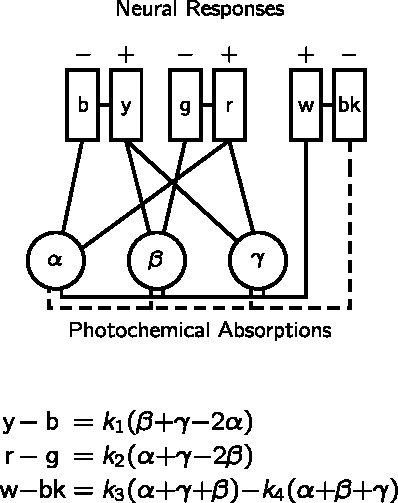
\includegraphics[width=0.6\linewidth]{fyz_fig490.pdf}
      \caption{Nervovéspoje podle \uv{oponentní} teorie barevného vidění (\cite[s.~697]{Feynman01})}
      \label{fyz:fig490}
    \end{figure}

    Tím se nám nabízí zajímavá možnost. U žádného jiného smyslu, který umožňuje nějaká měření,
    nedochází před vstupem do nervu k tak velkému množství procesů, jež by bylo možné nazvat
    výpočty. Pro všechny ostatní smysly probíhají výpočty v samotném mozku, kde je tolik vzájemných
    spojů, že dostat se na určité místo a provést tam měření, je téměř nemožné. U zrakového smyslu
    máme světlo, tři vrstvy buněk vykonávajících výpočty a výsledek se přenáší zrakovým nervem. Máme
    proto první možnost fyziologicky pozorovat, jak asi pracují první vrstvy mozku při svých
    krocích. Je to dvojnásob zajímavé, nejen z hlediska vidění, ale i z hlediska celkové fyziologie.

    Skutečnost, že existují tři pigmenty neznamená, že musí být tři druhy vjemů. Jiná teorie
    barevného vidění má zcela protikladná schémata uspořádání barev (obr. \ref{fyz:fig490}). Podle
    ní jedno z nervových vláken přenáší hodně impulsů, když oko vidí žlutou barvu a málo impulsů,
    když vidí modrou. Další nervové vlákno přenáší stejným způsobem zelenou a červenou informaci a
    další bílou a černou. Jinak řečeno, někdo se již pokusil odhadnout způsob připojení a metodu
    výpočtu.

    Problémy, jež bychom rádi vyřešili odhadem těchto výpočtů, souvisí s otázkou zdánlivých barev,
    které vidíme na růžovém podkladě, tím, co se stane, když se oko adaptuje na různé barvy a
    otázkou tzv. psychologických jevů. Psychologickými jevy jsou například takové jevy, jako že
    bílou „necítíme „jako červenou, žlutou a modrou. Tato teorie barevného vidění dále pokročila,
    protože psychologové tvrdí, že existují čtyři zdánlivé čisté barvy: „Existují čtyři stimuly, jež
    mají pozoruhodnou schopnost vyvolat psychologicky jednoduché barvy: modrou, žlutou, zelenou a
    červenou. Na rozdíl od žlutohnědé, červenohnědé, purpurové nebo od většiny odlišitelných barev
    jsou tyto jednoduché barvy nesmísené v tom smyslu, že žádná z nich se nezúčastňuje na podstatě
    druhé; přesněji modrá není nažloutlá, načervenalá nebo nazelenalá atd.; jsou to psychologicky
    primární barvy.“ To nazýváme psychologickým faktem. Abychom zjistili, na základě, čeho se došlo
    k tomuto konstatování, musíme opravdu těžko hledat v celé odborné literatuře. Vše, co o tom
    najdeme v moderní literatuře, je opakování toho, co jsme citovali. Případně bývá citován jistý
    německý psycholog, pro nějž je uznávanou autoritou Leonardo da Vinci, který, jak všichni dobře
    víme, byl velký umělec. Říká: „Leonardo si myslel, že existuje pět barev.“ Hledáme-li dál, v
    ještě starší knize najdeme takový důkaz: „Purpurová je červeno - modrá, oranžová je červeno -
    žlutá, ale můžeme vidět červenou jako purpurovo - oranžovou? Není červená a modrá jednodušší než
    purpurová nebo oranžová? Průměrná osoba, které se zeptáte, jaké jsou jednoduché barvy, vám
    vyjmenuje červenou, žlutou a modrou, tyto tři a někteří pozorovatelé dodají ještě čtvrtou,
    zelenou. Psychologové si zvykli považovat tyto čtyři za významné barvy.“ Taková je tedy situace
    v psychologické analýze věci. Když každý říká, že jsou tři, tak jsou tři, a když někdo řekne, že
    jsou čtyři a oni chtějí, aby byly čtyři, tak budou čtyři. Na tom jsou vidět těžkosti
    psychologického výzkumu. Je jasné, že máme takové pocity, ale informace o nich lze získat jen
    velmi těžko.

    Druhým směrem, kterým se můžeme ubírat, je směr fyziologický, to je experimentálně zjistit, co
    se ve skutečnosti děje v mozku, v oku, v sítnici nebo kdekoliv a můžeme objevit, že se po
    určitých nervových vláknech přenášejí určité kombinace impulzů z různých buněk. Mimochodem,
    primární pigmenty se nemusí nacházet v oddělených buňkách; mohou být buňky, jež obsahují směsi
    různých pigmentů, buňky s červeným a zeleným pigmentem, buňky, kde jsou všechny tři pigmenty
    (informace od všech tří je pak informace o bílé barvě) atd. Existuje mnoho způsobů, jak lze celý
    systém poskládat a na nás je, abychom objevili, jak je to v přírodě. Nakonec, můžeme mít naději,
    že pochopíme-li fyziologické souvislosti, potom aspoň zčásti pochopíme psychologické aspekty, o
    nichž jsme mluvili. Proto se podíváme tímto směrem.

  \section{Fyziologie oka}\label{fyz:IchapXXXVIsecII}
    Abychom si připomněli propojení uvnitř sítnice, znázorněné na obr. \ref {fyz:fig131}, nebudeme
    mluvit jen o barevném vidění, ale o vidění obecně. Sítnice je ve skutečnosti jako povrch mozku.
    I když skutečný obraz, jak ho vidíme mikroskopem, je o něco komplikovanější než tento
    schématický náčrt, můžeme při pozorné analýze vidět všechna vzájemná spojení. Nejsou
    pochybnosti, že jedna část povrchu sítnice je spojena s druhými částmi a že informace, jež se
    šíří v dlouhých axonech k nervovým buňkám, jsou kombinace informací z mnoha buněk. Jsou zde tři
    vrstvy buněk s navazujícími funkcemi: buňky sítnice, jež jsou ovlivňovány světlem, intermediální
    buňky, které přebírají informace od jednotlivých nebo od několika buněk sítnice a odevzdávají je
    buňkám v třetí vrstvě, odkud se přenášejí do mozku. Buňky v těchto vrstvách jsou křížově
    propojeny všemi možnými směry.
    
    \begin{figure}[ht!] %\ref{fyz:fig491}
      \centering
      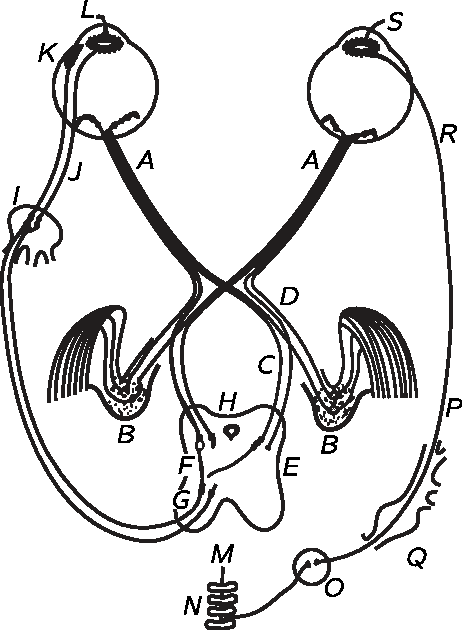
\includegraphics[width=0.8\linewidth]{fyz_fig491.pdf}
      \caption{Nervové mezispojení pro mechanické ovládání očí (\cite[s.~697]{Feynman01})}
      \label{fyz:fig491}
    \end{figure}

    Nyní přejdeme k některým stránkám struktury a činnosti oka (viz obr. \ref {fyz:fig130a}).
    Zaostřování světla se uskutečňuje hlavně rohovkou, díky jejímu zakřivenému povrchu, na němž se
    paprsky lámou. Proto nevidíme dobře pod vodou, neboť ve vodě nemáme dostatečný rozdíl mezi
    indexy lomu rohovky, který je roven \num{1.37} a vody, jenž je \num{1.33}. Za rohovkou je
    tekutina s indexem lomu téměř \num{1.33} a pak čočka, která má velmi zajímavou strukturu: skládá
    se ze série vrstev jako cibule, jenomže je celá průhledná. Uprostřed má index lomu \num{1.40} a
    na krajích \num{1.38}. (Bylo by dobré, kdybychom uměli vyrobit optické sklo s proměnlivým
    indexem lomu. Pak bychom nemuseli zakřivovat povrch čoček, jako to musíme dělat při konstantním
    indexu.) Navíc rohovka nemá tvar kulové plochy. U sférické čočky se projevuje určitá sférická
    aberace. Rohovka je na okrajích „plošší“ než kulová čočka, takže má menší sférickou aberaci.
    Pomocí systému rohovka -čočka se světlo zaostřuje na sítnici. Při pohledu na blízké a
    vzdálenější předměty se čočka napíná nebo uvolňuje, čímž přizpůsobuje ohnisko různým
    vzdálenostem. K přizpůsobení oka celkovému množství světla slouží duhovka, podle níž udáváme
    barvu očí jednotlivých osob - hnědou, modrou apod. Když se množství světla zvětšuje nebo
    zmenšuje, duhovka se stahuje nebo rozšiřuje. 
    
    Podívejme se na nervový systém, jenž řídí akomodaci čočky, pohyby oka, svaly, jež pohybují okem
    a duhovkou a který je schematicky znázorněn na obr. \ref{fyz:fig491}. Největší část informace,
    jež vychází z oka po optickém nervu A, se rozdělí do dvou svazků (o nichž ještě bude řeč) a tak
    jde do mozku. Několik vláken, které nás nyní zajímají, však nejde přímo do vizuálního centra v
    mozku, kde „vidíme“ obrazy, ale místo toho jdou do mezimozku (H). Jimi se měří osvětlení a
    nastavuje se clona duhovky, když je obraz rozmazaný, snaží se zkorigovat čočky, nebo když je
    obraz rozdvojený, snaží se nastavit oči na binokulámí vidění. Procházejí mezimozkem a zpětně se
    napojují na oko. K jsou svaly, jež ovládají akomodaci čoček a L jsou další svaly, jež jsou
    napojeny na duhovku. Duhovka má dva systémy svalů. Jeden tvoří kruhový sval L, který při
    podráždění duhovku stahuje a uzavírá. Jeho činnost je velmi rychlá a je přímo spojen s mozkem
    prostřednictvím krátkých axonů. Druhý, opačně působící systém, tvoří radiální svaly, takže, když
    se setmí a kruhový sval se uvolní, radiální svaly duhovku rozevřou. Zde se setkáváme, jako na
    mnoha jiných místech v těle, s několika svaly, jež působí v opačných směrech. V každém takovém
    případě je nervový systém ovládající svaly velmi jemně vyvážen, takže, když se vyšle signál, aby
    se jeden sval stáhnul, automaticky se vysílá i signál k uvolnění druhého svalu. Duhovka je v tom
    vzácnou výjimkou: nervy, jež způsobují stažení duhovky, jsme si již popsali, ale o nervech,
    které způsobují její roztažení, nikdo neví, odkud přesně přicházejí. Vedou někam dolů do míchy v
    hrudní části páteře, z míchy vedou vzhůru krčními gangliemi zpět do hlavy, aby nakonec ovládly
    zpětný pohyb duhovky. Vskutku, tento signál prochází zcela jiným nervovým systémem, vůbec ne
    centrálním, ale sympatickým nervovým systémem. Je to velmi divný způsob zabezpečení správné
    funkce.
    
    \begin{figure}[ht!] %\ref{fyz:fig492}
      \centering
      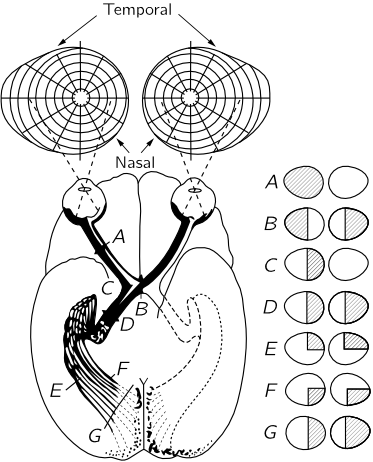
\includegraphics[width=1\linewidth]{fyz_fig492.png}
      \caption{Nervové spojení očí se zrakovým centrem (\cite[s.~697]{Feynman01})}
      \label{fyz:fig492}
    \end{figure}

    Další zvláštní věc týkající se oka jsme si již jednou zdůraznili. Jde o to, že buňky citlivé na
    světlo jsou na opačné straně, takže světlo musí projít několika vrstvami jiných buněk, než se
    dostane k receptorům - vnitřní strana je obrácena směrem ven! Vidíme, že některé vlastnosti oka
    jsou podivuhodné a některé jsou zdánlivě hloupé.

    Obrázek \ref{fyz:fig492} znázorňuje spojení mezi očima a částí mozku, která má přímý vztah k
    procesu vidění. Ihned za bodem D vnikají vlákna zrakových nervů do určité zóny nazvané
    \emph{geniculatum laterale}, odkud jdou do části mozku nazvané kůrové zrakové centrum. Všimněme
    si, že část vláken jde z každého oka do opačné části mozku, takže vytvořený obraz je neúplný.
    Zrakové nervy z levé části pravého oka procházejí optickým křížem (chiasma opticum) B a
    přidávají se k nim nervy z levé části levého oka. Takže levá část mozku dostává všechny
    informace přicházející z levé části každého oka, tj. z pravé části vizuálního pole, zatímco
    pravá strana mozku vidí levou část vizuálního pole. Tak se skládají informace z každého oka k
    určení vzdálenosti objektů. V tom spočívá binokulární systém vidění.

    Spojení mezi sítnicí a zrakovým centrem jsou velmi zajímavá. Poškodí-li se část sítnice, celé
    nervové vlákno odumře a podle toho můžeme zjistit, kde bylo připojeno. Ukazuje se, že v principu
    jde o spojení jedna k jedné - každému bodu na sítnici odpovídá jeden bod v zrakovém centru a
    body, jež jsou velmi blízko sebe na sítnici, jsou blízko sebe i v zrakovém centru. Zrakové
    centrum tak ještě stále odpovídá prostorovému seskupení tyčinek a čípků, i když už značně
    zdeformovanému. Body, jež jsou ve středu pole, a jsou na sítnici soustředěny na velmi malé
    ploše, jsou v zrakovém centru rozloženy na velmi mnoho buněk. Je vhodné, když věci, které jsou
    původně těsně vedle sebe, zůstanou vedle sebe i nadále. Nejzajímavější stránka celé věci je však
    tato: Místo, kde se zdá, že je nejdůležitější, aby věci zůstaly těsně vedle sebe, by bylo přesně
    ve středu vizuálního pole. I když se to zdá neuvěřitelné, svislá čára jdoucí středem našeho
    zrakového pole je taková, že informace z bodů ležících napravo od ní jdou do levé části mozku a
    informace z bodů ležících od ní nalevo jdou do pravé strany mozku. A tato střední oblast je
    rozdělena svislým řezem přímo uprostřed, takže věci, které jsou si ve středu velmi blízké, jsou
    od sebe v mozku velmi vzdálené! Takže informace z jedné části mozku se musí nějak dostávat do
    druhé části, což je dost překvapující.

    Velmi zajímavá je otázka, jak je celá tato síť propojena. Zde je starý problém, týkající se
    toho, co je již propojeno a co se teprve spojí učením, zkušeností. Někdy dříve se učilo, že
    přesné spojení ani není potřebné, stačí, když existují hrubé spoje a pak na základě zkušeností
    se malé dítě naučí, že když se věc nachází „tam“, vyvolá to určité pocity v mozku. (Lékaři nám
    vždy rádi říkají, co dítě „cítí“, ale jak vědí, co cítí dítě, když je mu jeden rok?) Lze
    předpokládat, že roční dítě vidí nějaký předmět „tam“, má určité pocity a učí se sáhnout „tam“,
    protože, když sáhne „sem“, předmět nenahmatá. Takový přístup pravděpodobně není správný, protože
    vidíme, že v mnoha případech již existují hotová detailní spojení. Mnohem více světla vrhají na
    věc některé pozoruhodné experimenty s mloky. (Shodou okolností mlok má přímé křížové spojení bez
    optického kříže, protože oči, které má každé na jedné straně hlavy, nemají společnou část
    zorného pole. Mlok nemá binokulární vidění.) Lze provést následující experiment. Přetneme-li
    mlokovi zrakový nerv, nerv z očí opět naroste. Tisíce a tisíce buněk vláken se tak opět spojí. U
    zrakového nervu nezůstávají vlákna jedno u druhého - je to jako velký spletený telefonní kabel,
    kde se všechna vlákna kroutí a překrývají, ale když se dostanou do mozku, všechna se opět
    uspořádají. Vzniká otázka: Když se mlokovi protne zrakový nerv, napojí se vůbec někdy správně?
    Odpověď je pozoruhodná: Ano. Protneme-li mlokovi nerv a ten opět naroste, má mlok opět dobrou
    zrakovou ostrost. Protneme-li však zrakový nerv, oko obrátíme vzhůru nohama a necháme opět
    přirůst, má mlok znovu dobrý ostrý zrak, ale je tady jedna osudná chyba: Když mlok vidí mouchu
    „tam nahoře“, skočí za ní „tam dolů“ a nikdy se to správně nenaučí. Jde tu proto o jakýsi
    záhadný způsob, kterým si tisíce vláken v mozku najdou své správné místo.

    Otázka počtu daných a získávaných spojů je důležitá pro teorii vývoje živočichů. Odpověď není
    známa, ale problematika se intenzivně zkoumá.
    
    Stejný experiment provedený s karasem zlatým ukazuje, že na místě, kde jsme nerv přesekli,
    vznikne nepěkný uzel jako velká jizva, ale přesto všechna vlákna srostou tak, že spojují správná
    místa mozku.
    
    Aby se to mohlo uskutečnit, jak rostou nová vlákna ve starých kanálech zrakového nervu, musí se
    nějak rozhodovat, kterým směrem mají růst. Jak to dělají? Zdá se, že záhada rozdílného růstu
    různých vláken je chemické povahy. Představme si obrovské množství rostoucích vláken, z nichž
    každé se něčím liší od svých sousedů, a přitom roste tak, že si najde své jediné správné místo
    pro konečné spojení s mozkem! Přitom zřejmě reaguje individuálním způsobem na nějaký neznámý
    chemický podnět. To je velmi zajímavá, přímo fantastická věc. Je to jeden z největších nedávných
    objevů biologie a nepochybně souvisí s mnoha dávnými nevyřešenými problémy růstu, organizace a
    vývoje organizmů a hlavně embryí.

    Další zajímavý jev souvisí s pohyby očí. Oči se musí pohybovat tak, aby jejich dva obrazy za
    různých okolností splývaly. Tyto pohyby jsou různého druhu. Jeden spočívá ve sledování něčeho,
    co si vyžaduje, aby se oči současně pohybovaly ve stejném směru, vpravo nebo vlevo, další pohyb
    je směřuje na stejné místo při různých vzdálenostech od očí, což vyžaduje protiběžné pohyby očí.
    Nervy ovládající oční svaly jsou propojeny tak, že jsou k těmto pohybům přizpůsobeny. Jeden druh
    nervů způsobuje stahy svalů na vnitřní straně jednoho oka a na vnější straně druhého oka a
    současně uvolní svaly na opačných stranách, takže oči se pohybují současně. Vzruch z dalšího
    centra způsobí, že oči se vychýlí z rovnoběžného směru směrem k sobě. Každé oko se může otočit k
    vnějšímu koutku, když se druhé oko pohybuje k nosu, ale je nemožné, ať už vědomě nebo nevědomě,
    otočit obě oči současně k vnějším koutkům. Ne proto, že by na očích nebyly takové svaly, ale
    proto, že neexistuje způsob, jak vyslat signál, že se mají obě oči otočit směrem ven. Výjimkou
    může být úraz nebo porušený nerv. I když svaly jednoho oka jím mohou volně pohybovat, ani jogín
    nedokáže vytočit současně obě oči směrem ven, neboť, jak se zdá, nejsme k tomu přizpůsobení.
    Naše nervová spojení jsou do jisté míry zafixována. To je důležitý fakt, protože většina starších
    knih o anatomii a psychologii neuznává nebo nezdůrazňuje skutečnost, že naše nervová spojení
    jsou do takové míry zafixována - tvrdí, že vše je jen naučené.

  \section{Tyčinky}\label{fyz:IchapXXXVIsecIII}
    Podívejme se pozorněji, co se děje v tyčinkách. Obr. \ref{fyz:fig493} znázorňuje střed tyčinkové
    buňky při pohledu elektronovým mikroskopem (tyčinka vyčnívá ze zorného pole). Mnoho vrstev je
    složeno z rovinných útvarů, zvětšeně je vidíme vpravo. Obsahují látku rhodopsin, barvu nebo
    pigment, jenž vyvolává zrakový efekt v tyčinkách. Pigment rhodopsin je protein obsahující
    zvláštní skupinu  nazvanou retinal, kterou můžeme oddělit od proteinu, a která je nepochybně
    hlavní příčinou absorpce světla. Důvod existence rovinných útvarů neznáme, ale je velmi
    pravděpodobné, že existuje nějaký důvod, proč musí být rhodopsinové molekuly uloženy rovnoběžně.
    Po chemické stránce je tato problematika dobře rozpracována, ale může se tu uplatnit i fyzika je
    možné, že všechny molekuly jsou seřazeny do jakési řady, takže, je-li některá z nich vypuzena,
    elektron, jenž se při tom uvolní, proletí celou řadou až dolů, aby signál vyšel ven, případně
    něco podobného. To je velmi důležitý, zatím však nevyřešený problém. Uplatnit se zde může
    biochemie i fyzika pevných látek.

    \begin{figure}[ht!] %\ref{fyz:fig493}
      \centering
      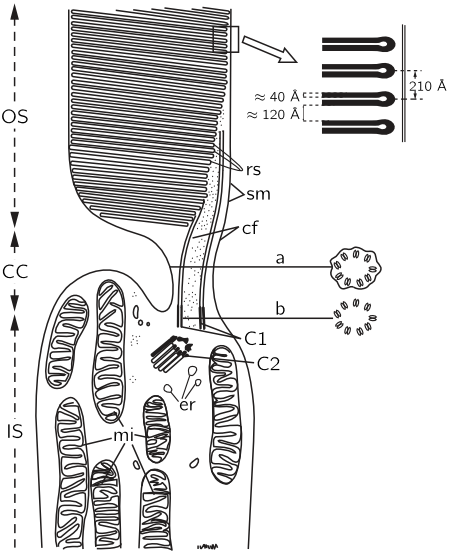
\includegraphics[width=1\linewidth]{fyz_fig493.png}
      \caption{Elektronová mikrografie tyčinkových buněk (\cite[s.~697]{Feynman01})}
      \label{fyz:fig493}
    \end{figure}

    Takovou vrstevnatou strukturu můžeme najít i jinde, kde je důležité světlo, například u
    chloroplastu v rostlinách, kde světlo způsobuje fotosyntézu. Při zvětšení tam najdeme téměř
    stejné vrstvy, jen v rostlinách je místo retinalu chlorofyl. Chemická struktura retinalu je
    znázorněna na obr. \ref{fyz:fig494}. V bočním řetězci obsahuje sérii střídajících se dvojných
    vazeb, což je charakteristické pro téměř všechny silně absorbující organické látky jako je
    chlorofyl, krev atd.je to látka, kterou si člověk nedokáže vytvořit ve svých vlastních buňkách -
    musíme ji přijímat potravou. Proto ji jíme ve formě zvláštní látky, jež je skoro stejná jako
    retinal, jen na pravém konci má ještě připojen vodík - je to vitamin A.je-li přísun tohoto
    vitamínu nedostatečný, máme málo retinalu a může se to projevit jako šeroslepost. Tehdy není v
    rhodopsinu dostatek pigmentu, abychom viděli v šeru pomocí tyčinek.

    \begin{figure}[ht!] %\ref{fyz:fig494}
      \centering
      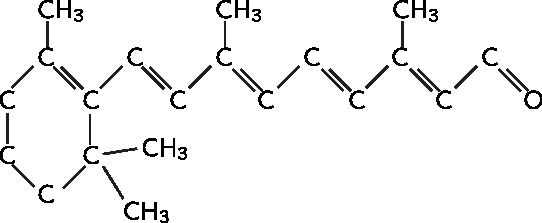
\includegraphics[width=1\linewidth]{fyz_fig494.pdf}
      \caption{Struktura retinalu (\cite[s.~697]{Feynman01})}
      \label{fyz:fig494}
    \end{figure}

    Důvod, proč takový řetězec dvojných vazeb silně absorbuje světlo, je také znám. Můžeme ho
    naznačit. Řada střídavých vazeb se nazývá konjugovanou dvojnou vazbou; dvojná vazba znamená, že
    tam je jeden elektron navíc a tento elektron se může velmi snadno přesunout doprava nebo doleva.
    Když na takovou molekulu dopadne světlo, elektrony v každé dvojné vazbě se posunou o jeden krok.
    Posunou se všechny elektrony v celém řetězci, jako když padají kostky domina postavené do řady,
    a i když se každá posune jen o kousek (očekáváme, že vjednom atomu se může elektron posunout
    pouze o malou vzdálenost), ale výsledný efekt je stejný, jakoby se elektron posunul z jednoho
    konce až na druhý konec! Je to totéž, jako by se jeden elektron pohyboval sem a tam po celém
    řetězci. Proto vlivem elektrického pole vzniká mnohem silnější absorpce, než kdybychom mohli
    posunout elektron jen o vzdálenost odpovídající jednomu atomu. Retinin velmi silně absorbuje
    světlo, neboť elektrony tak lze snadno posouvat. Takový je tady fyzikálněchemický mechanizmus.

  \section{Složené oko hmyzu}\label{fyz:IchapXXXVIsecIV}
    Vraťme se nyní do biologie. Lidské oko není jediným druhem oka. Téměř všichni obratlovci mají
    oči podobné lidským. Nižší živočichové však mají mnoho jiných druhů očí: oční skvrny, různé oční
    pohárky a jiné méně citlivé orgány, o nichž nemáme čas hovořit. Mezi bezobratlými však existuje
    jeden druh vysoce vyvinutého oka, a to je \textbf{složené oko hmyzu}. (Většina hmyzu má vedle
    velkých složených očí ještě i různé dodatečné, jednodušší oči.) Velmi podrobně se zkoumal zrak
    včely. Vlastnosti včelího zraku lze snadno studovat, protože včely přitahuje med a lze připravit
    experimenty, kde se med odliší tak, že se položí na modrý nebo na červený papír a sleduje se, ke
    kterému včely přiletí. Takovou metodou se podařilo objevit několik velmi zajímavých věcí
    týkajících se vidění včel.

    \begin{figure*}[ht!] %\ref{fyz:fig495}
      \centering
      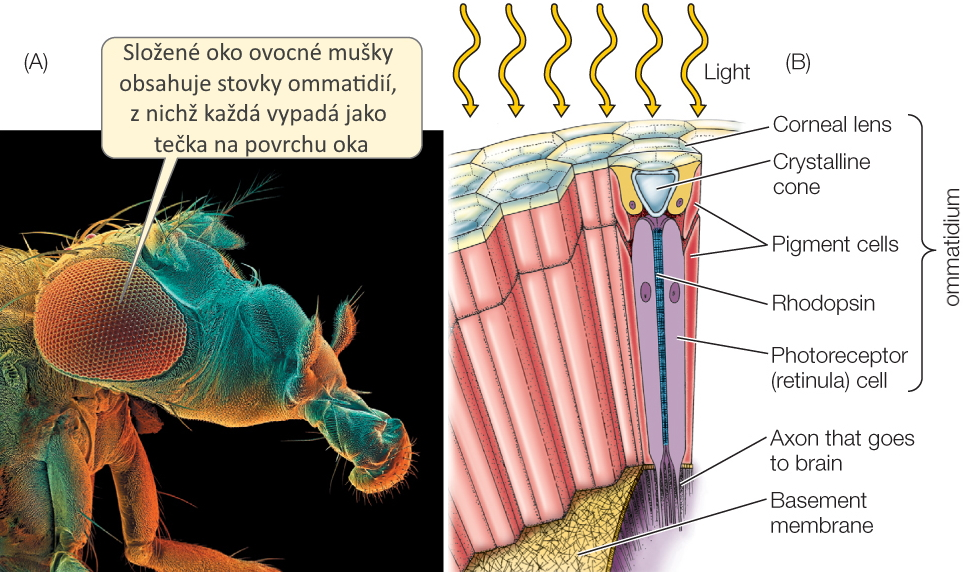
\includegraphics[width=1\linewidth]{fyz_fig495a.jpg}
      \caption{Struktura ommatidia (jednoduché buňky složeného oka) (\cite[s.~697]{Feynman01})}
      \label{fyz:fig495}
    \end{figure*}

    V první řadě musíme poznamenat, že při pokusech měřit, jak vidí včely rozdíl v barvě mezi dvěma
    „bílými“ papíry, zjistili někteří výzkumníci, že včely to příliš dobře neumí a jiní zjistili, že
    jsou v tom fantastické. I když byly dva kousky bílého papíru téměř úplně stejné, včely stále
    mohly poznat rozdíl mezi nimi. Experimentátoři použili na jednom papíru zinkovou bělobu a na
    druhém olověnou bělobu, a i když jsou obě barvy pro nás úplně stejné, včely je mohly stále
    rozeznat, neboť tyto barvy různě odrážejí světlo v ultrafialové oblasti (obr. \ref{fyz:fig921}).
    Tak se zjistilo, že včelí oko je citlivé v širším rozsahu spektra, než je náš rozsah. Naše oko
    vidí od \SI{700}{\nm} do \SI{400}{\nm}, od červené po fialovou, ale včelí oko vidí až do
    \SI{300}{\nm}, tj. po ultrafialovou oblast! Na základě toho vzniká mnoho zajímavých jevů. Za
    prvé, včely mohou rozlišit mnoho květů, které se nám zdají stejné. Samozřejmě, musíme si
    uvědomit, že barvy květů nejsou určeny pro naše oči, ale pro včelí - jsou to signály, které
    přitahují včely k určitým květům. Všichni víme, že existuje mnoho „bílých“ květů. Bílá barva
    není zřejmě pro včely příliš zajímavá, neboť se ukazuje, že všechny bílé květy různě odrážejí
    ultrafialové světlo. Neodrážejí ho na sto procent, jak by ho měla odrážet skutečná bílá. Ne
    všechno světlo se odráží zpět, ultrafialové chybí, to znamená, že vzniká nějaká barva, právě tak
    jako pro nás, když chybí modrá, světlo je žluté. Proto jsou pro včely všechny květy barevné. Ale
    také se zjistilo se, že včely nevidí červenou. Proto bychom mohli očekávat, že všechny červené
    květy jsou pro včelu černé, ale není tomu tak. Při podrobném studiu červených květů dokonce i
    naším okem můžeme postřehnout, že většina z nich má mírně namodralý nádech, protože dodatečně
    odrážejí ještě i modrou barvu, kterou včela vidí. Experimenty dále ukazují, že květy se liší i v
    tom, jak různé části jejich okvětních lístků odrážejí ultrafialové světlo atd. Kdybychom tedy
    mohli vidět květy tak, jak je vidí včely, byly by ještě krásnější a různorodější.

    \begin{figure}[ht!] %\ref{fyz:fig921}
      \centering
      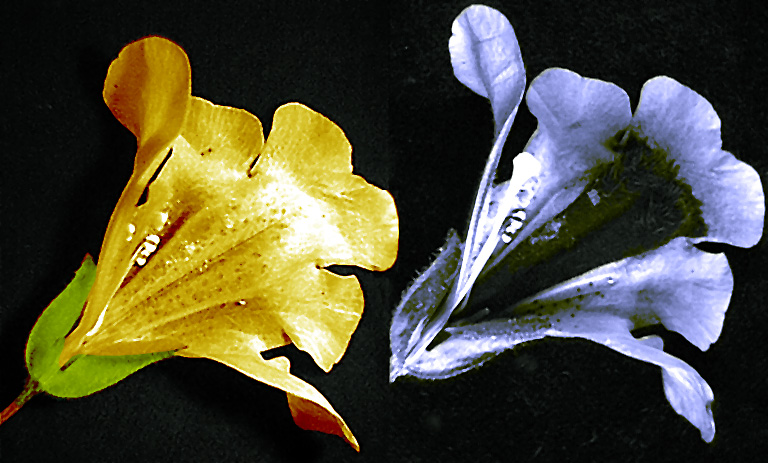
\includegraphics[width=1\linewidth]{fyz_fig921.jpg}
      \caption{Květina fotografovaná pod bílým a UV světlem.}
      \label{fyz:fig921}
    \end{figure}
    
    Bylo zjištěno, že existují takové červené květy, které neodrážejí modré nebo ultrafialové
    světlo, takže včelám se budou zdát černé! To velmi zaujalo odborníky zabývající se těmito věcmi,
    protože černá barva se zdá být nezajímavá, neboť je těžko odlišitelná od špinavého stínu.
    Skutečně se ukázalo, že se včely těmto květům vyhýbají, ale „navštěvují“ je kolibříci a ti
    červenou vidí!

    Další zajímavou stránkou zraku včel je, že při pohledu na kousek modrého nebe umí včela určit
    směr ke Slunci, aniž by ho viděla. My to tak snadno nedokážeme. Když se podíváme z okna na nebe
    a vidíme, že je modré, kterým směrem se nachází Slunce? Včela to pozná, protože je dost citlivá
    k polarizaci světla a rozptýlené světlo oblohy je polarizované.
    
    Říká se také, že včela postřehne blikání až do frekvence 200 cyklů za sekundu, zatímco my jen do
    20. Pohyby včel v úlu jsou velmi rychlé. Včely pohybují nohama a vibrují křídly, ale tyto pohyby
    lze velmi těžko postřehnout naším okem. Kdybychom však viděli mnohem rychleji, tyto pohyby
    bychom pozorovali. Pro včelu je asi velmi důležité, aby její oko mělo tak rychlý postřeh. 
    
    Podívejme se, jakou ostrost vidění můžeme předpokládat u včely. její oko je složené, vytvořené z
    velkého množství zvláštních buněk nazvaných ommatidia. Jsou uspořádána kuželovitě na kulové
    ploše na vnější části hlavy včely. Jedno omatidium je na obr. \ref{fyz:fig495}.  Nahoře se
    nachází průhledná část, druh jakési „čočky“, ale ve skutečnosti je to spíš filtr nebo světelná
    trubice, která přivádí světlo podél tenkého vlákna, kde pravděpodobně dochází k absorpci. Z
    druhého konce vychází nervové vlákno. Centrální vlákno je obklopeno šesti buňkami, které ho
    kryjí. Takový popis pro naše účely stačí. Hlavní je, že omatidium je kuželovitý útvar a že se
    jich vejde na povrchu včelího oka vedle sebe velmi mnoho.

    \begin{figure}[ht!] %\ref{fyz:fig496}
      \centering
      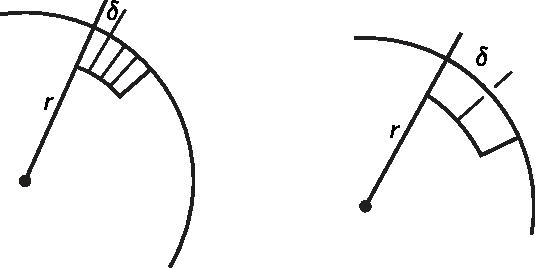
\includegraphics[width=1\linewidth]{fyz_fig496.pdf}
      \caption{Schéma umístění ommatidií v oku včely (\cite[s.~697]{Feynman01})}
      \label{fyz:fig496}
    \end{figure}

    Nyní se podívejme na rozlišovací schopnost včelího oka. Nakreslíme-li čáry znázorňující
    ommatidia na povrchu koule s poloměrem \(r\) (0b. \ref{fyz:fig496}), můžeme vypočítat šířky
    každého ommatidia. Použijeme k tomu náš rozum a budeme předpokládat, že vývoj je stejně chytrý
    jako my je-li ommatidium velmi velké, rozlišovací schopnost bude malá. Jedna buňka získá
    informaci z jednoho směru a vedlejší buňka z nějakého jiného směru atd., a co je mezi tím, to
    včela dobře neuvidí. Takže neurčitost zrakové ostrosti oka bude určitě souviset s nějakým úhlem
    - s úhlem příslušejícím jednomu ommatidiu - mezi krajním směrem ommatidia a směrem ke středu
    křivosti oka. (Zrakové buňky jsou, samozřejmě, pouze na povrchu koule, uvnitř je hlava včely.)
    Tento úhel od jednoho ommatidia k druhému je roven poměru průměru ommatidia a poloměru oka

    \begin{equation}\label{fyz:eq682}
      \Delta\alpha_g = \frac{\delta}{r}
    \end{equation}

    Takže bychom mohli říct, „čím bude \(\delta\) menší, tím bude lepší zraková ostrost oka. Proč
    potom nemá včela velmi tenoučká ommatidia?“ Odpověď je následující. Z fyziky již víme dost k
    tomu, abychom si uvědomili, že chceme-li světlo dostat do úzké štěrbiny, uplatní se ohybové jevy
    a v daném směru nebudeme dobře vidět. Vzhledem k difrakci tam může vnikat světlo z různých směrů
    z celkového úhlu \(\alpha_d\) takového, že
    
    \begin{equation}\label{fyz:eq587}
      \Delta\alpha_d = \frac{\lambda}{\delta}
    \end{equation}    

    \begin{figure}[ht!] %\ref{fyz:fig497}
      \centering
      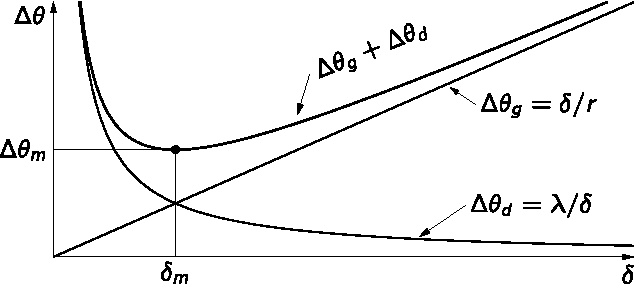
\includegraphics[width=1\linewidth]{fyz_fig497.pdf}
      \caption{Optimální velikost ommatidia je \(\delta_m\) (\cite[s.~697]{Feynman01})}
      \label{fyz:fig497}
    \end{figure}

    Nyní vidíme, že bude-li \(\delta\) příliš malé, nebude vzhledem k difrakci každé ommatidium
    vidět jen v jednom směru. Budou-li ommatidia příliš velká, uvidí každé v určitém směru, ale
    nebude jich dost k tomu, aby vytvořily dobrý obraz dané scény. Proto vzdálenost \(\delta\)
    nastavíme tak, abychom optimalizovali vliv obou účinků. Sečteme-li je a najdeme minimum tohoto
    součtu (obr. \ref{fyz:fig495}), máme
    \begin{equation}\label{fyz:eq588}
      \frac{d(\Delta\alpha_g + \Delta\alpha_d}{\delta} = 0 = \frac{1}{r} - \frac{\delta}{\lambda^2}.
    \end{equation}     
    odtud plyne vzdálenost
    \begin{equation}\label{fyz:eq589}
      \delta = \sqrt{\lambda\cdot r}.
    \end{equation} 
    Odhadneme-li, že \(r\) je kolem 3 milimetrů a za vlnovou délku světla, které vidí včela, vezmeme
    \SI{400}{\nm}, máme
    \begin{equation}\label{fyz:eq590}
      \delta = \sqrt{\num{3e-3}\cdot\num{4e-7}}\si{\m} = \SI{3.5e-5}{\m} = \SI{35}{\micro\m}.
    \end{equation} 

    Podle literatury je to \SI{30}{\micro\m}, což je v dobrém souhlasu s naším odhadem, a tedy
    chápeme, čím je určena velikost včelího oka! Lze postupovat i opačně, vycházet z tohoto čísla a
    zjistit, jaká je rozlišovací schopnost včelího oka. Ve srovnání s naší je velmi slabá. Ve
    porovnání se včelou jsme schopni uvidět předměty, jejichž zdánlivá velikost je třicetkrát menší.
    Ve srovnání s námi vidí včela dost rozmazaně a neostře. Přesto je to v pořádku a je to nejlepší,
    co může být. Můžeme se zeptat, proč nemá včela dobré oči jako my s čočkou atd. Je k tomu několik
    zajímavých důvodů. Za prvé, včela je příliš malá, a kdyby měla takové oko jako my, ale v měřítku
    svých rozměrů, otvor oka by měl kolem \SI{30}{\micro\m} a difrakce by se projevovala tak silně,
    že by jím i stejně neviděla dobře. Oko není dobré, je-li příliš malé. Za druhé, kdyby bylo tak
    velké jako včelí hlava, byla by celá hlava obsazena okem. Krása složeného oka je v tom, že
    nepotřebuje prostor, je to jen velmi tenká vrstva na povrchu včely. Takže, když tvrdíme, že ho
    mají mít takové jako my, musíme si připomenout, že i včely mají své vlastní problémy!

  \section{Jiné oči}\label{fyz:IchapXXXVIsecV}
    Kromě včel vidí barvu i mnozí jiní živočichové. Ryby, motýli, ptáci a plazi mohou vidět barvu,
    ale předpokládá se, že většina savců ji vidět nemůže. Primáti ji mohou vidět. Ptáci barvu určitě
    vidí a to souvisí i se zbarvením ptáků. Bylo by zbytečné, aby samečkové byli tak krásně
    zbarvení, kdyby to samičky nemohly ocenit! Takže vývoj pohlavního nebo jiného vybavení, které
    mají ptáci, je výsledkem toho, že samičky jsou schopny vidět barvy. Až se příště podíváme na
    páva a zamyslíme se nad bohatstvím a jemností jeho zbarvení, měli bychom vzdát hold ne pávovi,
    ale pávici za její zrakovou ostrost a estetický smysl, neboť ten inspiroval takovou nádhernou
    podívanou!

    \begin{figure}[ht!] %\ref{fyz:fig498}
      \centering
      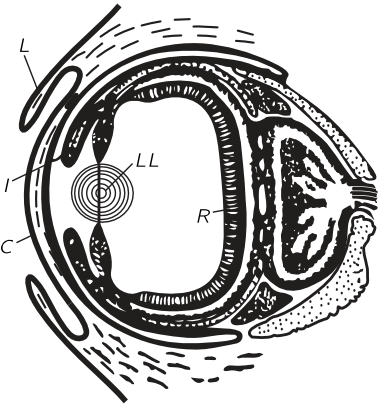
\includegraphics[width=0.8\linewidth]{fyz_fig498.png}
      \caption{Oko chobotnice (\cite[s.~697]{Feynman01})}
      \label{fyz:fig498}
    \end{figure}

    Všichni bezobratlí mají slabě vyvinuté oči nebo složené oči, ale všichni obratlovci mají oči
    podobné našim, až na jednu výjimku. Když myslíme na nejvyšší formu živočichů, obvykle říkáme: To
    jsme my, ale když přistoupíme na méně předpojaté hledisko a omezíme se jen na bezobratlé, k nimž
    nepatříme a zeptáme se, který z nich je nejvyšší živočich, většina zoologů bude souhlasit s tím,
    že je to chobotnice! Velmi zajímavé je to, že kromě vyvinutého mozku a reakcí, jež jsou pro
    bezobratlé velmi dobré, má ještě i samostatně vyvinuté oko. Není to složené oko nebo oční skvrna
    - má rohovku, víčko, duhovku, má čočku, má dvě oblasti naplněné tekutinou a vzadu má sítnici. V
    podstatě je to stejné jako u obratlovců! Je to zajímavý příklad koincidence v evoluci, kde
    příroda našla dvakrát totéž řešení problému, jen s malým vylepšením. Překvapivě se ukazuje, že
    sítnice chobotnice je také částí mozku, jež se oddělila v embryonálním vývoji od mozku stejně
    jako u obratlovců, ale odlišné a zajímavé je to, že buňky citlivé na světlo jsou na vnitřní
    straně a buňky, které „dělají výpočty“, jsou za nimi, opačně než u našeho oka. Tak aspoň vidíme,
    že pro otočení naší sítnice vnitřkem ven není nějaký vážný důvod. (Viz obr. \ref{fyz:fig494})
    Krakatice obrovská má největší oči na světě. Našli se už i takové oči, které měly průměr až 38
    cm!
  
  \section{Neurologie zraku}\label{fyz:IchapXXXVIsecVI}
    Jeden z hlavních bodů našeho předmětu je otázka propojení informací z jedné části oka s druhou
    částí. Podívejme se na složené oko ostrorepa amerického, s nímž byly provedeny pozoruhodné
    experimenty. Nejdříve si musíme uvědomit, jaké informace se mohou přenášet prostřednictvím
    nervů. Nerv přenáší určitý vzruch, jenž má elektrické účinky a je snadné je detekovat je to
    vzruch podobný vlně, která se šíří podél nervu a vyvolává nějaké účinky na jeho druhém konci.
    Informace se šíří podél dlouhé části nervové buňky, nazvané axon, ve formě určitého hrotovitého
    pulzu. Šíří-li se po nervu jeden pulz, nemůže hned po něm následovat další. Všechny pulzy mají
    stejnou velikost, takže při větším dráždění nedostaneme větší pulzy, ale za sekundu jejich víc.
    Velikost pulzuje určena nervovým vláknem. To je důležité si uvědomit, abychom viděli, co se děje
    dále. 
    
    Na obrázku \ref {fyz:fig499a} je složené oko ostrorepa amerického. Oku se moc nepodobá, má jen
    kolem tisíce ommatidií. Na obrázku \ref {fyz:fig499b}  je průřez oka. Jsou tam vidět ommatidia s
    nervovými vlákny, které z nich vycházejí do mozku. Všimněme si, že dokonce i u ostrorepa je málo
    mezispojů. Jsou mnohem jednodušší než v lidském oku, a to nám umožňuje studovat jednodušší
    případ.

    \begin{figure}[hb!] %\ref{fyz:fig499}
      \centering
      \subcaptionbox{normální pohled \label{fyz:fig499a}}{\luafigure[0.9]{fyz_fig499a.jpg}} \newline
      \subcaptionbox{průřez \label{fyz:fig499b}}{\luafigure[0.9]{fyz_fig499b.jpg}}
      \caption{Složené oko ostrorepa amerického (\cite[s.~601]{Feynman01}).}
      \label{fyz:fig499}
    \end{figure}

    Nyní se podívejme na experimenty, jež byly provedeny pomocí jemných elektrod napojených na
    optické nervy ostrorepa při osvětlení pouze jednoho ommatidia, což lze snadno realizovat pomocí
    čoček. Zapneme-li v nějakém čase \(t_0\) světlo a měříme vycházející elektrické signály,
    zjistíme, že nejprve je krátká pauza a za ní následuje série pulzů, které se postupně ustálí, a
    následují v pravidelných intervalech jak je to na obr. \ref {fyz:fig500a}. Když světlo vypneme,
    signály se ztratí. Zajímavé je, že necháme-li zesilovač napojen na týž nerv a osvítíme jiné
    ommatidium, nic se nestane, nevzniknou žádné signály.

    \begin{figure}[hb!] %\ref{fyz:fig500}
      \centering
      \subcaptionbox{\label{fyz:fig500a}}{\luafigure[1]{fyz_fig500a.pdf}}  \newline
      \subcaptionbox{\label{fyz:fig500b}}{\luafigure[1]{fyz_fig500b.pdf}}  
      \caption{Reakce nervových vláken oka ostrorepa amerického na světlo (\cite[s.~601]{Feynman01}).}
      \label{fyz:fig500}
    \end{figure}

    Nyní provedeme jiný experiment. Osvítíme původní ommatidium a dostaneme to, co předtím. Když
    však nyní osvítíme i jiné blízké ommatidium, pulzy se na chvíli přeruší a pak pokračují v mnohem
    pomalejším rytmu (obr. \ref{fyz:fig500b}). Rytmus jednoho je zpomalen pulzy, které přicházejí z
    druhého! Každý nerv tedy přenáší signály z jednoho ommatidia, ale jejich množství je ovlivněno
    signály z ostatních ommatidií. Když je tedy celé oko téměř rovnoměrně osvětleno, bude informace
    přicházející z jednoho ommatidia relativně slabá, neboť je brzděna ostatními. Toto přibrzdění je
    aditivní. Neboť osvítíme-li mnoho blízkých omatidií, bude zbrzdění velké. Pro blízká ommatidia
    je tedy přibrzdění velké a pro ta, jež jsou dost daleko, je prakticky nulové. Takže je aditivní
    a závisí na vzdálenosti. To je první příklad toho, jak se kombinují informace z různých částí
    oka už v samotném oku. Když o tom trochu přemýšlíme, vidíme, že je to asi zařízení k zesílení
    kontrastu na obrysech předmětů, neboť, je-li část obrazu světlá a část černá, dávají ommatidia v
    osvětlené části pulzy zeslabované okolním světlem, takže jsou relativně slabé. Zato ommatidium,
    jež je zaměřeno na okraj předmětu, a ještě dostává světlo, je přibrzďováno okolními, ale těch
    není mnoho, neboť některá z nich jsou tmavá. Výsledný signál je proto silnější. Výsledek bude
    dán křivkou na obr. \ref{fyz:fig501}. Ostrorep bude vidět zvýrazněný obrys předmětu.
    
    Fakt, že dochází k zvýraznění obrysů, je znám již dávno. Je to zajímavý jev, který psychologové
    mnohokrát komentovali. Abychom nakreslili předmět, stačí, když nakreslíme jeho obrysy. Jak jsme
    zvyklí se dívat na obrázky, které mají jen obrysy! Co jsou to obrysy? Obrys je jen rozdíl na
    okraji mezi světlem a tmou nebo mezi dvěma barvami. Není to nic určitého. Třeba se zdá
    neuvěřitelné, ale vůbec to neznamená, že každý předmět má kolem sebe čáru! Taková čára
    neexistuje. Existuje jen v našem psychologickém založení - začínáme rozumět tomu, proč stačí
    čára, abychom dostali klíč k celé věci. Lze předpokládat, že naše oči pracují podobným způsobem
    - mnohem komplikovanějším, ale podobným.

    \begin{figure}[ht!] %\ref{fyz:fig501}
      \centering
      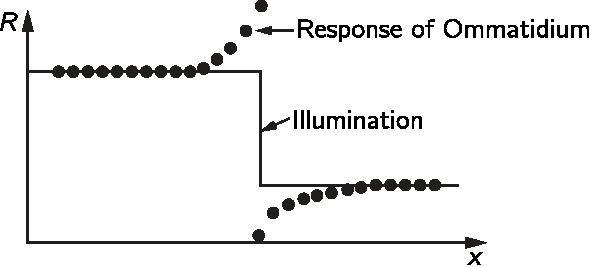
\includegraphics[width=0.6\linewidth]{fyz_fig501.pdf}
      \caption{
              (\cite[s.~697]{Feynman01})}
      \label{fyz:fig501}
    \end{figure}

    Nakonec stručně popíšeme pěkný, rozsáhlejší a pokročilejší výzkum, který se prováděl se žábami.
    Pomocí velmi jemných elektrod zasunutých do optických nervů žáby můžeme získat signály, které
    postupují jen daným axonem, podobně jako tomu bylo u ostrorepa. Na základě analogického
    experimentu zjistíme, že tato informace nezávisí jen na jednom místě v oku, ale je součtem
    informací z více míst.
    
    Poslední experimenty studující funkci žabího oka jsou následující. Můžeme najít čtyři druhy
    nervových vláken odpovídajících čtyřem druhům reakcí. Tyto experimenty se neprovádějí zapínáním
    a vypínáním světelných pulzů, protože to žába nevidí. Žába si prostě sedí a její oči se vůbec
    nehýbají, pokud se nepohne list leknínu a v tom případě kývá očima přesně tak, že obraz se
    nemění. Jinak žába oči neotáčí. Když se něco pohybuje v jejím zorném poli, například malý
    brouček (musí být schopna vidět něco malého pohybujícího se na pevném pozadí), ukáže se, že má
    čtyři druhy vláken, které přenášejí informaci. Jejich vlastnosti jsou shrnuty v tabulce 36.1.
    Udržovaná detekce rozhraní (nevymazatelná) znamená, že posuneme-li do zorného pole žáby předmět
    s okrajem v tomto vlákně, vznikne mnoho pulzů, které trvají, dokud Se předmět pohybuje, ale
    klesnou na udržovanou hodnotu, když je okraj už v zorném poli, i když se nepohybuje. Vypneme-li
    světlo, pulzy zmizí. Když ho opět zapneme, dokud je okraj ještě v zorném poli, opět se obnoví.
    Další druh vlákna je velmi podobný, ale nereaguje, je-li okraj přímý. Musí být vypouklý s tmavým
    pozadím! Jak komplikovaný musí být systém mezispojení v sítnici žabího oka, aby rozeznal, že do
    zorného pole vstoupil vypouklý předmět! Dále, i když toto vlákno částečně udržuje signály, není
    to tak dlouho jako u prvního vlákna a při vypnutí a Opětovném zapnutí světla se signály už
    neobnoví. Závisí na pohybu vypouklého předmětu v zorném poli. Oko ho vidí vstupovat dovnitř a
    pamatuje si, že tam je, ale stačí, když na chvíli vypneme světlo, zapomene na něj a už ho
    nevidí.

    \begin{table*}[hb!]
      \begin{tabular}{@{}lll@{}}
      \toprule
        \textbf{Typ}                                  & \textbf{Rychlost}            & \textbf{Úhlové pole} \\ \midrule
        1. Udržovaná detekce rozhraní (nevymazatelná) & \SIrange{0.2}{0.5}{\m\per\s} & \ang{1}              \\
        2. Detekce vypouklého rozhraní (vymazatelná)  & \SI{0.5}{\m\per\s}           & \ang{2} - \ang{3}    \\
        3. Detekce změny kontrastu                    & \SIrange{1}{2}{\m\per\s}     & \ang{7} - \ang{10}   \\
        4. Detekce stmívání                           & do \SI{12}{\m\per\s}         & do \ang{15}          \\
        5. Detekce tmy                                & ?                            & velmi velké          \\ \bottomrule
      \end{tabular}
      \caption{Typy reakcí optických vláken žáby}
    \end{table*}

    Další příklad se týká detekce změny kontrastu. Pohybuje-li se rozhraní dovnitř nebo ven,
    vznikají pulzy, ale když se nehýbe, žádné pulzy nevznikají. 
    
    Dále se v oku žáby nachází detektor stmívání. Klesá-li intenzita světla, generuje signály; když
    se však intenzita ustálí, signály přestanou. Detektor působí jen při stmívání.

    Nakonec je tam několik vláken, které slouží jako detektory tmy. Nejpřekvapivější na nich je, že
    neustále vyrábějí signály. Zvětšíme-li Osvětlení, následují signály řidčeji, ale neustanou. Když
    osvětlení zmenšíme, signály jsou častější. Ve tmě divoce kmitají a neustále říkají: \uv{Je tma!
    je tma! Je tma!}

    \begin{figure}[ht!] %\ref{fyz:fig502}
      \centering
      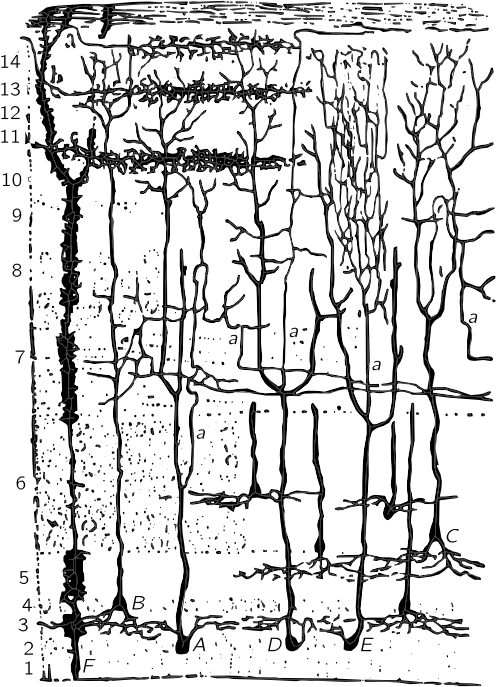
\includegraphics[width=1\linewidth]{fyz_fig502.png}
      \caption{Tectum žáby (\cite[s.~697]{Feynman01})}
      \label{fyz:fig502}
    \end{figure}

    Tyto reakce se zdají být dosti komplikované na to, aby bylo možné je klasifikovat a můžeme i
    pochybovat zda se experimenty správně interpretují. Proto je velice zajímavý poznatek, že takové
    čtyři druhy vláken je u žáby možno jasně anatomicky rozeznat! Po klasifikaci těchto reakcí byly
    realizovány jiné experimenty (je důležité, že až po provedení klasifikace), při nichž se
    zjistilo, že v různých vláknech není rychlost šíření signálů stejná, což umožňuje další
    nezávislou kontrolu toho, o které vlákno jde!
    
    Další zajímavou otázkou je, z jak veliké oblasti sbírá určité vlákno informaci. Zjistilo se, že
    tato oblast je různá pro různá vlákna.
    
    Obr. \ref{fyz:fig502} znázorňuje povrch nazvaný tectum žáby, kde vstupují vlákna zrakového nervu
    do mozku. Všechna nervová vlákna vytvářejí spojení v různých vrstvách tecta. Tato vrstvovitá
    struktura je podobná sítnici, a to je z části důvod, proč víme, že sítnice a mozek jsou si
    navzájem podobné. Vezmeme-li elektrodu a procházíme jí postupně různými vrstvami, můžeme
    zjistit, kde příslušná vlákna končí a dostaneme nádherný výsledek, že různé druhy vláken končí v
    různých vrstvách! První druh vlákna končí ve vrstvě prvního typu, druhý ve vrstvě druhého typu,
    třetí a pátý končí na stejném místě a nejhlouběji ze všech končí čtvrtý druh. (Jaká shoda
    okolností, že je očíslovali téměř ve správném pořadí? Není to tak, protože právě kvůli tomu je
    přečíslovali; v prvním článku byly očíslovány jinak!)
    
    Můžeme stručně shrnout, co jsme se naučili: Pravděpodobně existují tři pigmenty. Mohou existovat
    různé druhy receptorových buněk obsahujících tyto tři pigmenty v různých poměrech, ale existuje
    mnoho mezispojení, která dovolují sčítání a odčítání barev sčítáním a zesilováním signálů v
    nervovém systému. Takže dříve, než pochopíme barevné vidění, budeme muset pochopit výsledný
    vjem. je to stále otevřený problém, ale výzkumy pomocí mikroelektrod a podobných zařízení nám
    snad poskytnou víc informací o tom, jak vidíme barvy.

%---------------------------------------------------------------------------------------------------